% Options for packages loaded elsewhere
\PassOptionsToPackage{unicode}{hyperref}
\PassOptionsToPackage{hyphens}{url}
%
\documentclass[
  tikz]{standalone}
\usepackage{amsmath,amssymb}
\usepackage{iftex}
\ifPDFTeX
  \usepackage[T1]{fontenc}
  \usepackage[utf8]{inputenc}
  \usepackage{textcomp} % provide euro and other symbols
\else % if luatex or xetex
  \usepackage{unicode-math} % this also loads fontspec
  \defaultfontfeatures{Scale=MatchLowercase}
  \defaultfontfeatures[\rmfamily]{Ligatures=TeX,Scale=1}
\fi
\usepackage{lmodern}
\ifPDFTeX\else
  % xetex/luatex font selection
\fi
% Use upquote if available, for straight quotes in verbatim environments
\IfFileExists{upquote.sty}{\usepackage{upquote}}{}
\IfFileExists{microtype.sty}{% use microtype if available
  \usepackage[]{microtype}
  \UseMicrotypeSet[protrusion]{basicmath} % disable protrusion for tt fonts
}{}
\makeatletter
\@ifundefined{KOMAClassName}{% if non-KOMA class
  \IfFileExists{parskip.sty}{%
    \usepackage{parskip}
  }{% else
    \setlength{\parindent}{0pt}
    \setlength{\parskip}{6pt plus 2pt minus 1pt}}
}{% if KOMA class
  \KOMAoptions{parskip=half}}
\makeatother
\usepackage{xcolor}
\setlength{\emergencystretch}{3em} % prevent overfull lines
\providecommand{\tightlist}{%
  \setlength{\itemsep}{0pt}\setlength{\parskip}{0pt}}
\setcounter{secnumdepth}{-\maxdimen} % remove section numbering
\usepackage{tkz-fct}
\usepackage{tikz}
\usepackage{tkz-fct}
\usepackage{tkz-euclide}
\usepackage{tkz-tab}
\ifLuaTeX
  \usepackage{selnolig}  % disable illegal ligatures
\fi
\usepackage{bookmark}
\IfFileExists{xurl.sty}{\usepackage{xurl}}{} % add URL line breaks if available
\urlstyle{same}
\hypersetup{
  hidelinks,
  pdfcreator={LaTeX via pandoc}}

\author{}
\date{}

\begin{document}

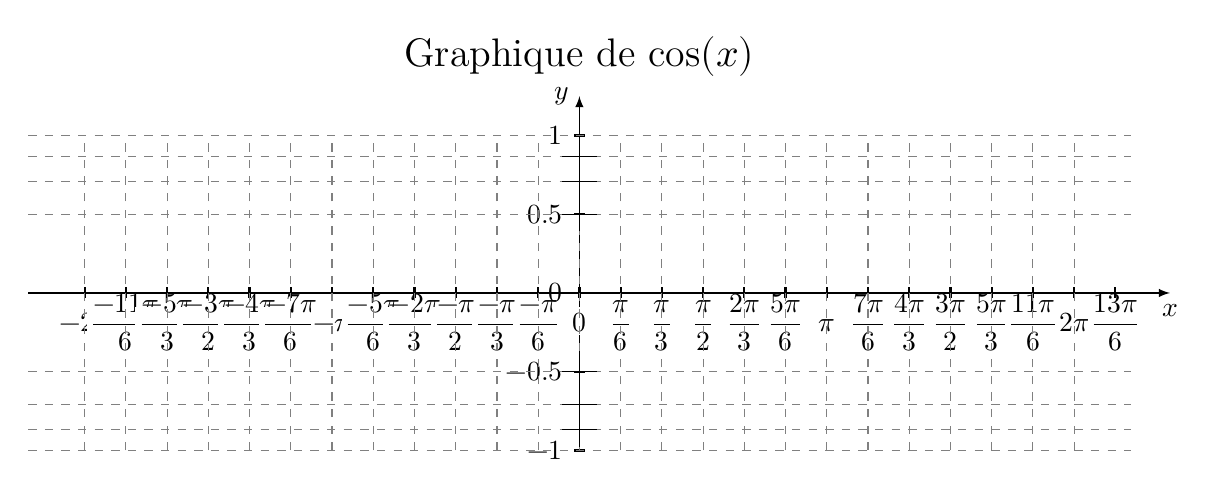
\begin{tikzpicture}

   \tkzInit[xmin=-7,xmax=7,ymin=-1,ymax=1, ystep=0.5]
\tkzAxeY
\tkzAxeX[trig=6]
  \foreach\v in {-1,-0.5,0.5,sqrt(2)/2,sqrt(3)/2,-sqrt(2)/2,-sqrt(3)/2,1}
  {\tkzHLine[dashed, color=gray]{\v}}
  \foreach\v in {-12,...,12}
  {\tkzVLine[dashed, color=gray]{\v*pi/6}}
 \tkzDefPoints{0/0.5/S1,0/0.70710678118/S2,0/0.86602540378/S3}
   \tkzDrawPoints[shape=cross,size=12](S1,S2,S3)

      \tkzDefPoints{0/-0.5/S1,0/-0.70710678118/S2,0/-0.86602540378/S3}
   \tkzDrawPoints[shape=cross,size=12](S1,S2,S3)

\tkzText(0,1.5){\Large Graphique de $\cos(x)$}

 \end{tikzpicture}

\end{document}
